\documentclass[tikz, border=2pt]{standalone}
\usepackage{tikz}
\begin{document}
    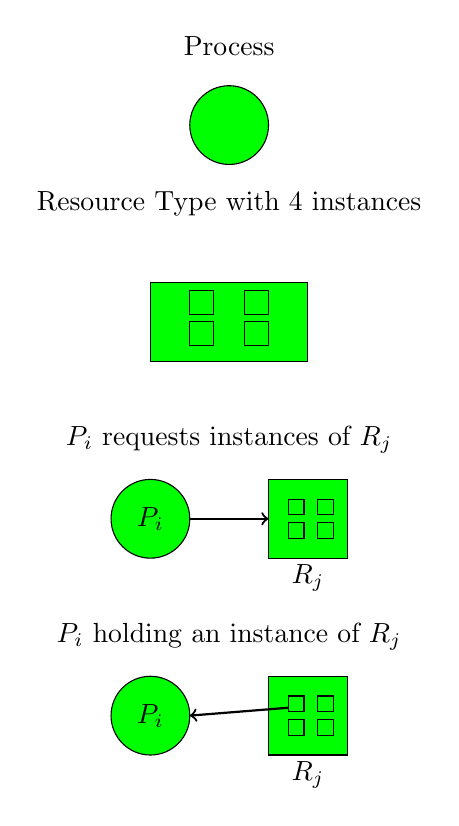
\begin{tikzpicture}
        \node at (0,16) {Process};
            \draw[fill=green] (0,15) circle (0.5);
        \node at (0,14) {Resource Type with 4 instances};
            \draw[fill=green] (-1,12) rectangle (1,13);
            \draw[fill=green] (-0.5, 12.6) rectangle ++(0.3, 0.3);
            \draw[fill=green] (0.5, 12.6) rectangle ++(-0.3, 0.3);
            \draw[fill=green] (0.5, 12.5) rectangle ++(-0.3, -0.3);
            \draw[fill=green] (-0.5, 12.5) rectangle ++(0.3, -0.3);
        \node at (0, 11) {$P_i$ requests instances of $R_j$};
            \draw[fill=green] (-1,10) 
                circle (0.5) 
                node {$P_i$};
            \draw[fill=green] (0.5,9.5)
                rectangle ++(1, 1);
            \node at (1, 9.25) {$R_j$};
            \draw[fill=green] (1.125, 9.75)
                rectangle ++(0.2, 0.2);
            \draw[fill=green] (1.125, 10.25)
                rectangle ++(0.2, -0.2);
            \draw[fill=green] (0.75, 10.25)
                rectangle ++(0.2, -0.2);
            \draw[fill=green] (0.75, 9.75)
                rectangle ++(0.2, 0.2);
            \draw[->, thick] (-0.5, 10) -- (0.5, 10);
        \node at (0,8.5) {$P_i$ holding an instance of $R_j$};
            \draw[fill=green] (-1,7.5) 
                circle (0.5) 
                node {$P_i$};
            \draw[fill=green] (0.5,7)
                rectangle ++(1, 1);
            \node at (1, 6.75) {$R_j$};
            \draw[fill=green] (1.125, 7.25)
                rectangle ++(0.2, 0.2);
            \draw[fill=green] (1.125, 7.75)
                rectangle ++(0.2, -0.2);
            \draw[fill=green] (0.75, 7.75)
                rectangle ++(0.2, -0.2);
            \draw[fill=green] (0.75, 7.25)
                rectangle ++(0.2, 0.2);
            \draw[->, thick] (0.75, 7.6) -- (-0.5, 7.5);
    \end{tikzpicture}
\end{document}